\documentclass[]{article}
\usepackage[round]{natbib}

\usepackage{fullpage}
\usepackage{listings}
\usepackage{url}
\usepackage{authblk}
\usepackage{graphicx}
\usepackage{color}
\usepackage{booktabs}

% lorem ipsum dummy text
\usepackage{lipsum}

\lstset{language=Python}

% cross-reference with main text
\usepackage{xr}
\externaldocument{doc}

% local definitions
\newcommand{\comment}[1]{{\textcolor{red}{Comment: #1}}}
\newcommand{\aprcomment}[1]{{\textcolor{blue}{APR: #1}}}

\usepackage{xspace}
\newcommand{\GEVA}{\texttt{GEVA}\xspace}
\newcommand{\tsdate}{\texttt{tsdate}\xspace}
\newcommand{\relate}{\texttt{Relate}\xspace}


\begin{document}
\title{Supporting Information for ``An article template''}
\author[*]{Aaron P. Ragsdale}
\affil[]{Kevin R. Thornton}
\affil[*]{apragsdale@wisc.edu}
\date{\today}
\maketitle

\renewcommand{\thefigure}{S\arabic{figure}}
\renewcommand{\thetable}{S\arabic{table}}
\renewcommand{\theequation}{S\arabic{equation}}
\setcounter{figure}{0}
\setcounter{table}{0}
\setcounter{equation}{0}

\section*{Supplemental methods}

\subsection*{Generation times needed to explain long-lasting differences between populations}

\subsection*{Allele ages from \GEVA}

\subsection*{Allele ages from \relate}

\subsection*{Allele ages from \tsdate}

\bibliographystyle{genetics}
\bibliography{doc}

\clearpage

\section{Tables and figures}

\begin{table}[h]
    \centering
    \begin{tabular}[t]{l|cccccc}
        \toprule
        Dataset & A$\rightarrow$C & A$\rightarrow$G & A$\rightarrow$T &
            C$\rightarrow$A & C$\rightarrow$G & C$\rightarrow$T \\
        \midrule
        \GEVA & 0.0946 & 0.3600 & 0.0886 & 0.1201 & 0.1057 & 0.2310 \\
        \tsdate & 0.0931 & 0.3579 & 0.0899 & 0.1146 & 0.1061 & 0.2384 \\
        \tsdate (w/singletons) & 0.0989 & 0.3598 & 0.0908 & 0.1168 & 0.1062 & 0.2275 \\
        \relate & 0.0991 & 0.3610 & 0.0863 & 0.1124 & 0.1038 & 0.2374 \\
        \relate (w/singletons) & 0.1002 & 0.3590 & 0.0921 & 0.1164 & 0.1060 & 0.2263 \\
        \midrule
        Trios (phased) & 0.0953 & 0.3649 & 0.0890 & 0.0960 & 0.1216 & 0.2332 \\
        Trios (all mutations) & 0.0962 & 0.3638 & 0.0923 & 0.0951 & 0.1202 & 0.2324 \\
        \bottomrule
    \end{tabular}
    \caption{
        \label{tab:recent-spectra}
        \textbf{Mutation profiles from the past 100 generations, compared to
        Iceland trios.} The most recent time bin for each method included the
        past $\approx150$ generations. When singletons were included (when
        using data from \tsdate and \relate), the spectra of estimated recent
        standing variation were unchanged. Note that \GEVA does not report ages
        for singletons.  While the three methods provide similar spectra from
        recent mutations, the spectrum from the Iceland pedigrees differs, in
        particular for the C$\rightarrow$A and C$\rightarrow$G classes. These
        differences are up to $2\%$ of the proportion among all mutations,
        which corresponds to an under- or over-count of up to $\sim20\%$ of
        C$\rightarrow$A and C$\rightarrow$G mutations, respectively.  This
        difference remains whether the spectrum is estimated from only
        mutations that were phased in \citet{jonsson2017parental} or from all
        mutations (phased and unphased).
    }
\end{table}

\begin{table}[h]
    \centering
    \begin{tabular}[t]{l|cccccc}
        \toprule
        Dataset & A$\rightarrow$C & A$\rightarrow$G & A$\rightarrow$T &
            C$\rightarrow$A & C$\rightarrow$G & C$\rightarrow$T \\
        \midrule
        AFR (\GEVA) & 0.103 & 0.354 & 0.094 & 0.127 & 0.098 & 0.224 \\
        EAS & 0.111 & 0.341 & 0.103 & 0.131 & 0.094 & 0.220 \\
        EUR & 0.102 & 0.355 & 0.093 & 0.125 & 0.102 & 0.222 \\
        SAS & 0.095 & 0.355 & 0.090 & 0.123 & 0.099 & 0.238 \\
        \midrule
        AFR (\relate) & 0.099 & 0.356 & 0.084 & 0.116 & 0.110 & 0.236 \\
        EAS & 0.095 & 0.359 & 0.089 & 0.115 & 0.097 & 0.245 \\
        EUR & 0.100 & 0.368 & 0.085 & 0.110 & 0.102 & 0.235 \\
        SAS & 0.104 & 0.344 & 0.090 & 0.108 & 0.107 & 0.246 \\
        \midrule
        AFR (\tsdate) & 0.092 & 0.354 & 0.087 & 0.116 & 0.110 & 0.241 \\
        EAS & 0.098 & 0.356 & 0.097 & 0.112 & 0.103 & 0.233 \\
        EUR & 0.091 & 0.363 & 0.089 & 0.117 & 0.102 & 0.238 \\
        SAS & 0.091 & 0.359 & 0.088 & 0.114 & 0.107 & 0.241 \\
        \bottomrule
    \end{tabular}
    \caption{
        \label{tab:recent-spectra}
        \textbf{Mutation profiles from the past 100 generations in continental
        population groups.}
    }
\end{table}



\begin{figure}[ht!]
    \centering
    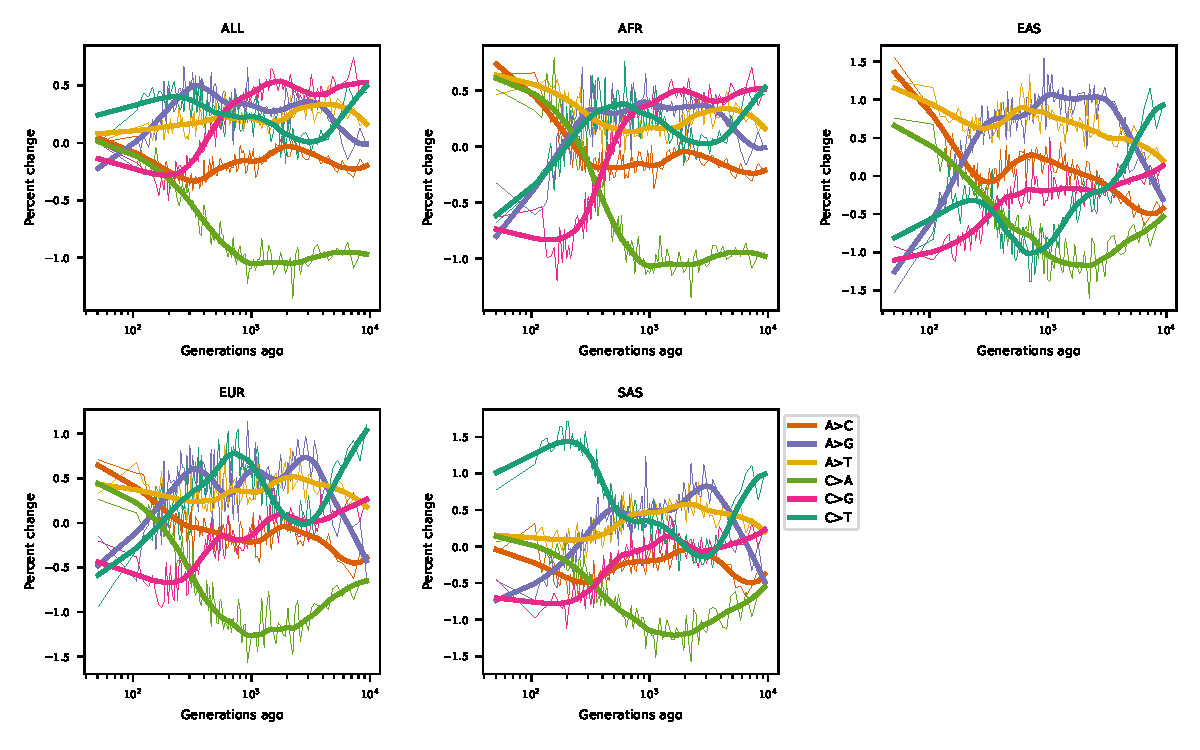
\includegraphics[width=\textwidth]{../plots/spectrum_history.geva.max_age.10000.pdf}
    \caption{
        \textbf{\GEVA-inferred mutation spectrum history.}
    }
    \label{fig:geva-spectra}
\end{figure}


\begin{figure}[ht!]
    \centering
    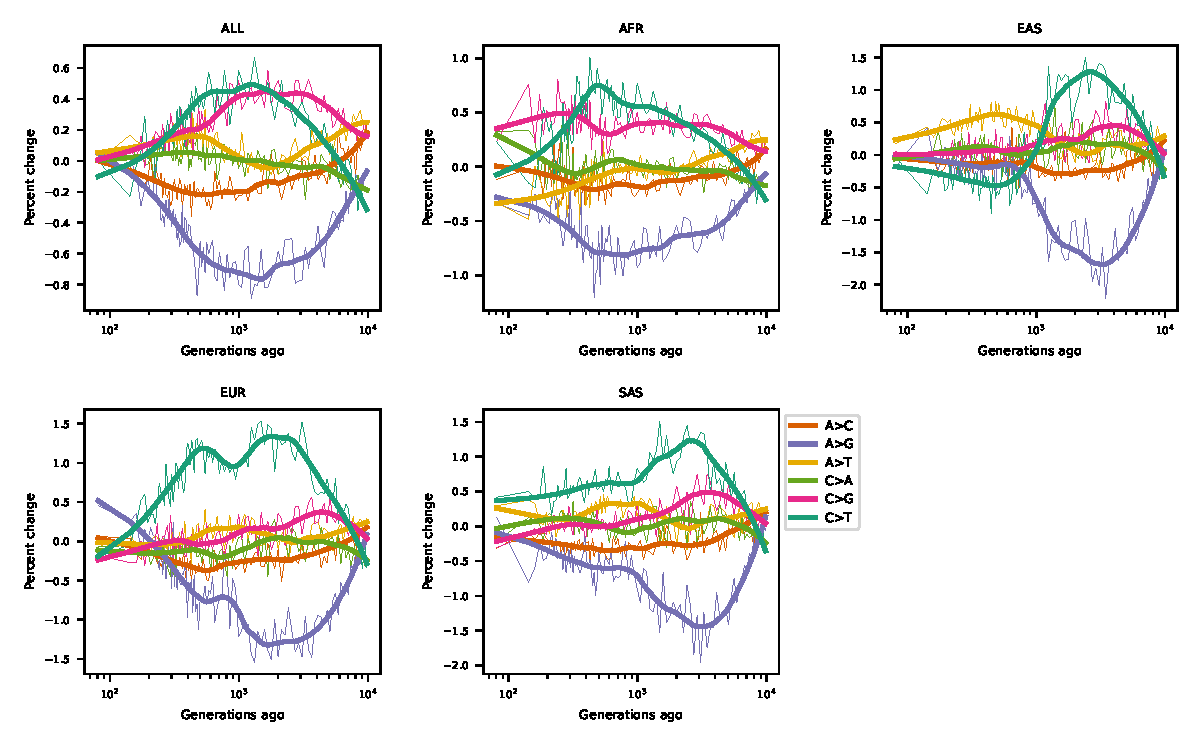
\includegraphics[width=\textwidth]{../plots/spectrum_history.relate.max_age.10000.pdf}
    \caption{
        \textbf{\relate-inferred mutation spectrum history.}
    }
    \label{fig:relate-spectra}
\end{figure}


\begin{figure}[ht!]
    \centering
    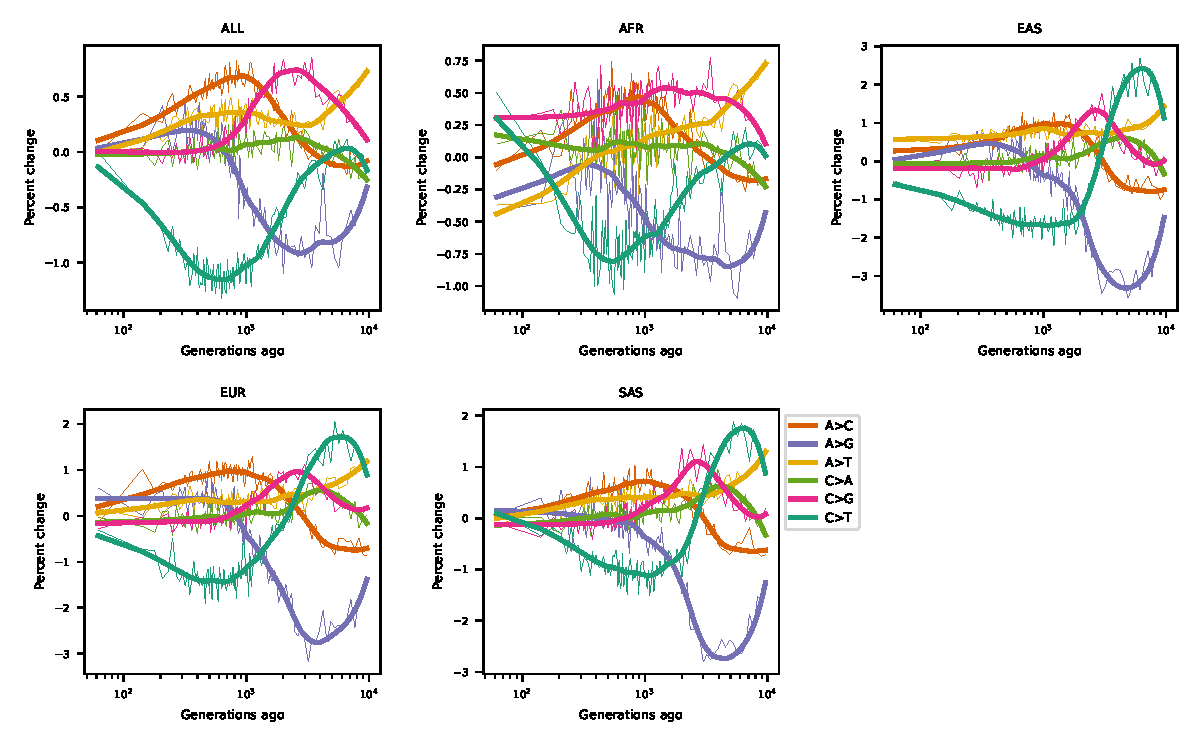
\includegraphics[width=\textwidth]{../plots/spectrum_history.tsdate.max_age.10000.pdf}
    \caption{
        \textbf{\tsdate-inferred mutation spectrum history.}
    }
    \label{fig:tsdate-spectra}
\end{figure}

\begin{figure}[ht!]
    \centering
    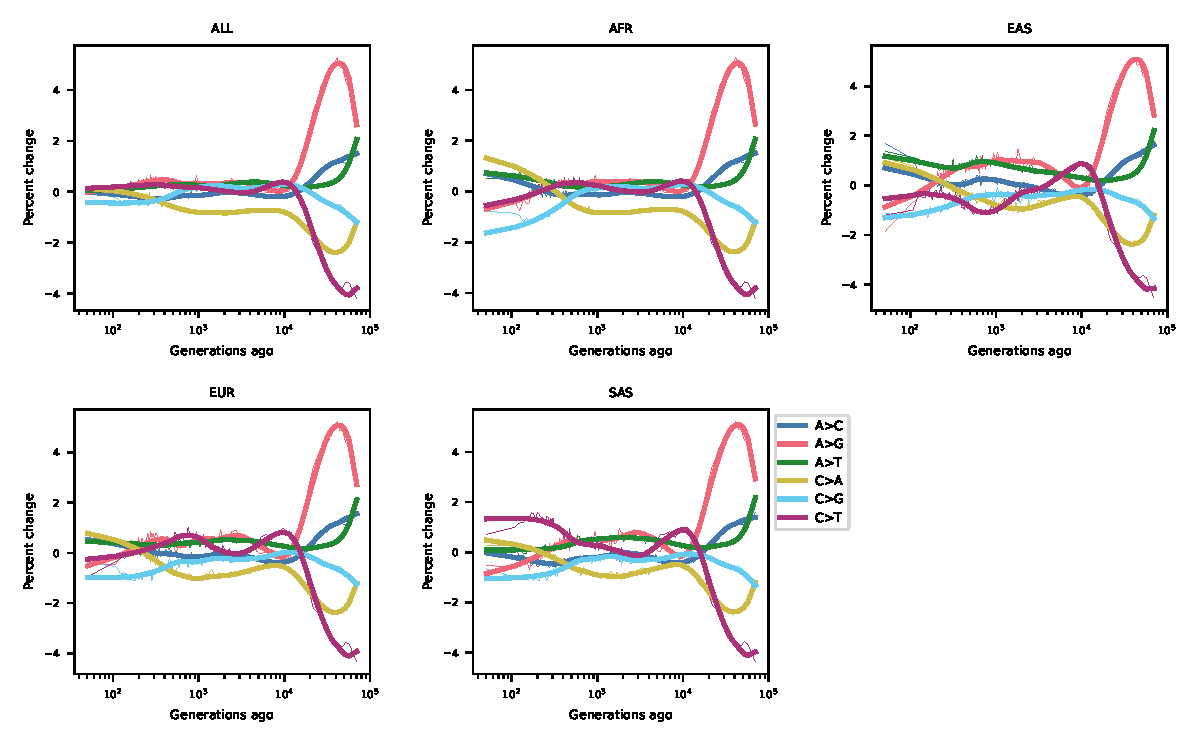
\includegraphics[width=\textwidth]{../plots/spectrum_history.geva.max_age.80000.pdf}
    \caption{
        \textbf{\GEVA-inferred mutation spectrum history, extending to 80,000 generations.}
    }
    \label{fig:geva-spectra-80k}
\end{figure}

\begin{figure}[ht!]
    \centering
    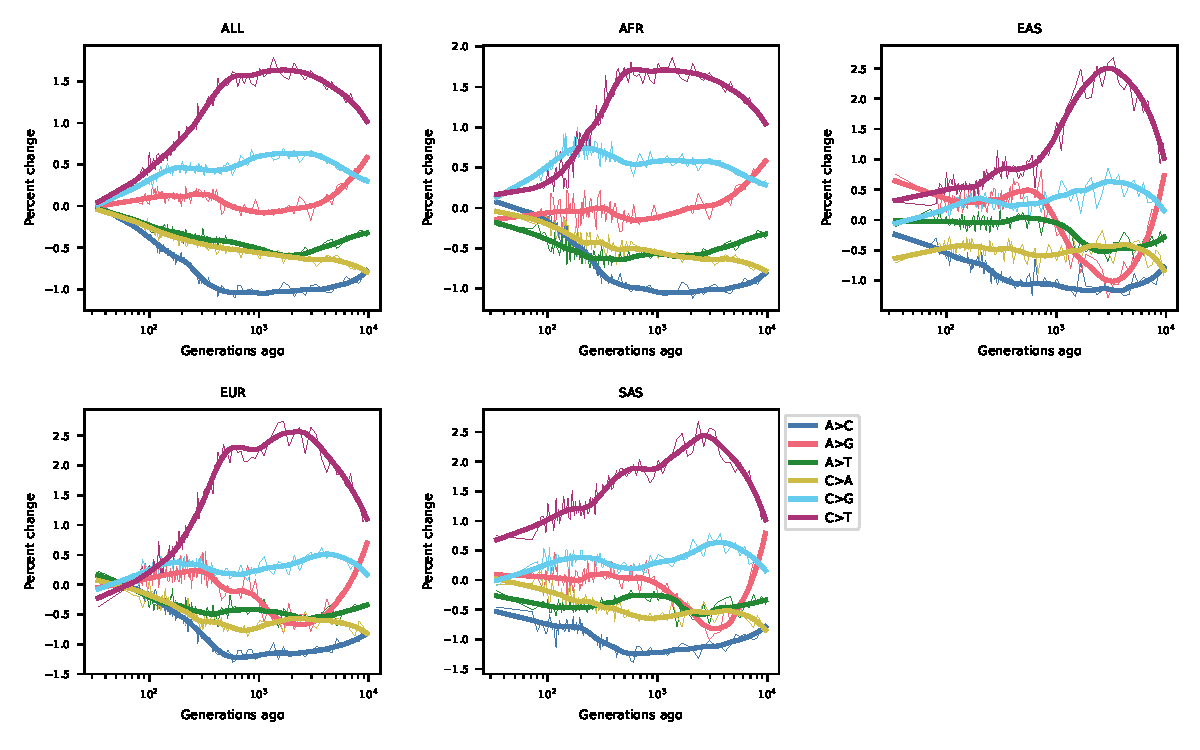
\includegraphics[width=\textwidth]{../plots/spectrum_history.relate.max_age.10000.singletons.pdf}
    \caption{
        \textbf{\relate-inferred mutation spectrum history, including singletons.}
    }
    \label{fig:relate-spectra-singletons}
\end{figure}


\begin{figure}[ht!]
    \centering
    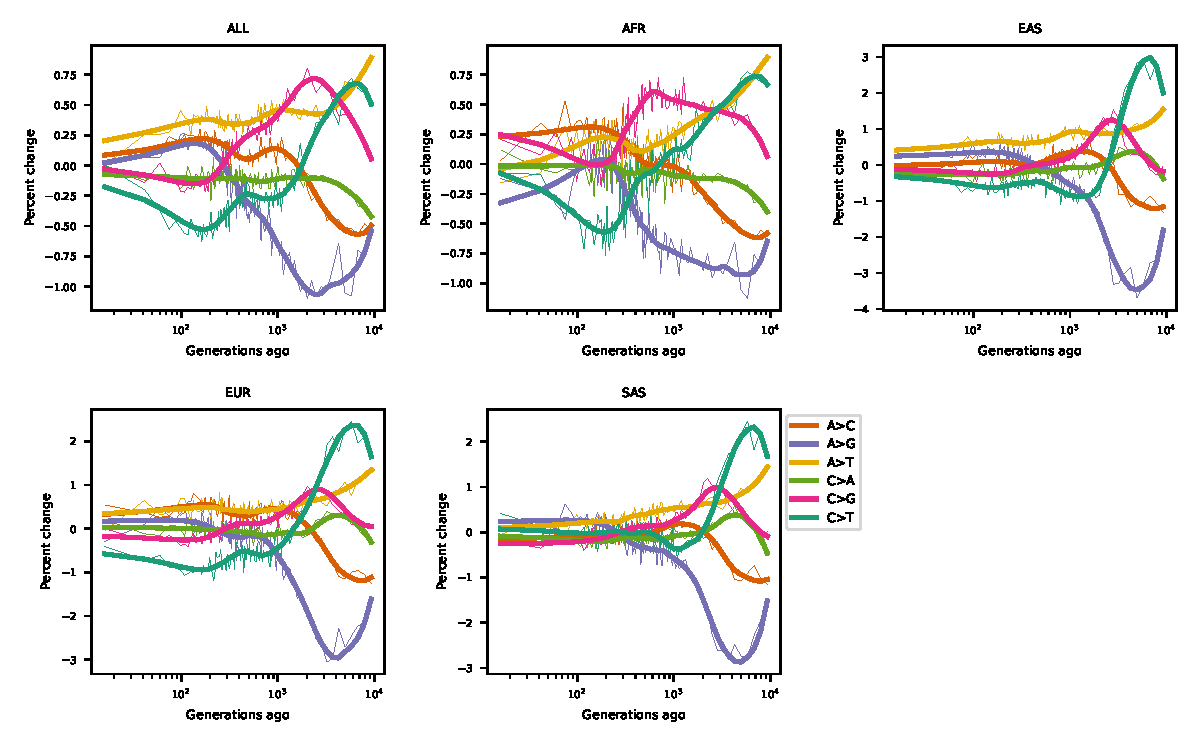
\includegraphics[width=\textwidth]{../plots/spectrum_history.tsdate.max_age.10000.singletons.pdf}
    \caption{
        \textbf{\tsdate-inferred mutation spectrum history, including singletons.}
    }
    \label{fig:tsdate-spectra-singletons}
\end{figure}


\begin{figure}[ht!]
    \centering
    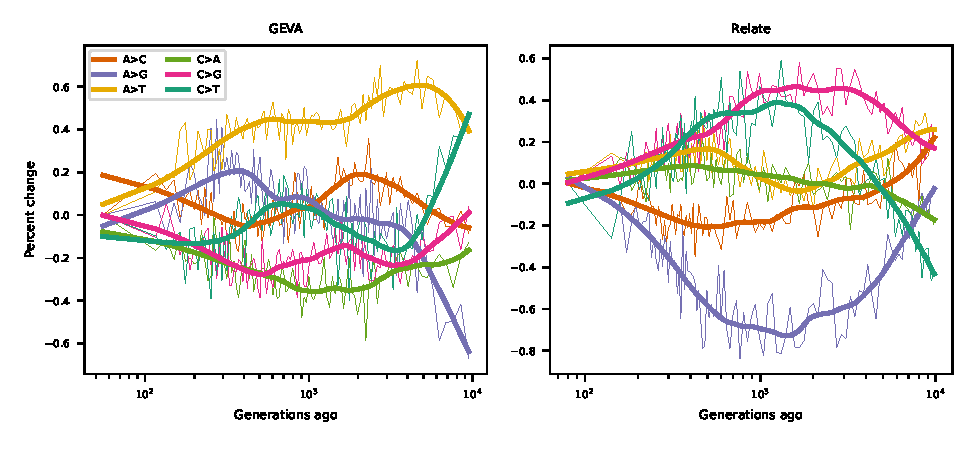
\includegraphics{../plots/overlapping.geva.relate.pdf}
    \caption{
        \textbf{Mutation spectrum histories from mutations that were dated by
        both \GEVA and \relate.}
    }
    \label{fig:overlap-spectra}
\end{figure}


\begin{figure}[ht!]
    \centering
    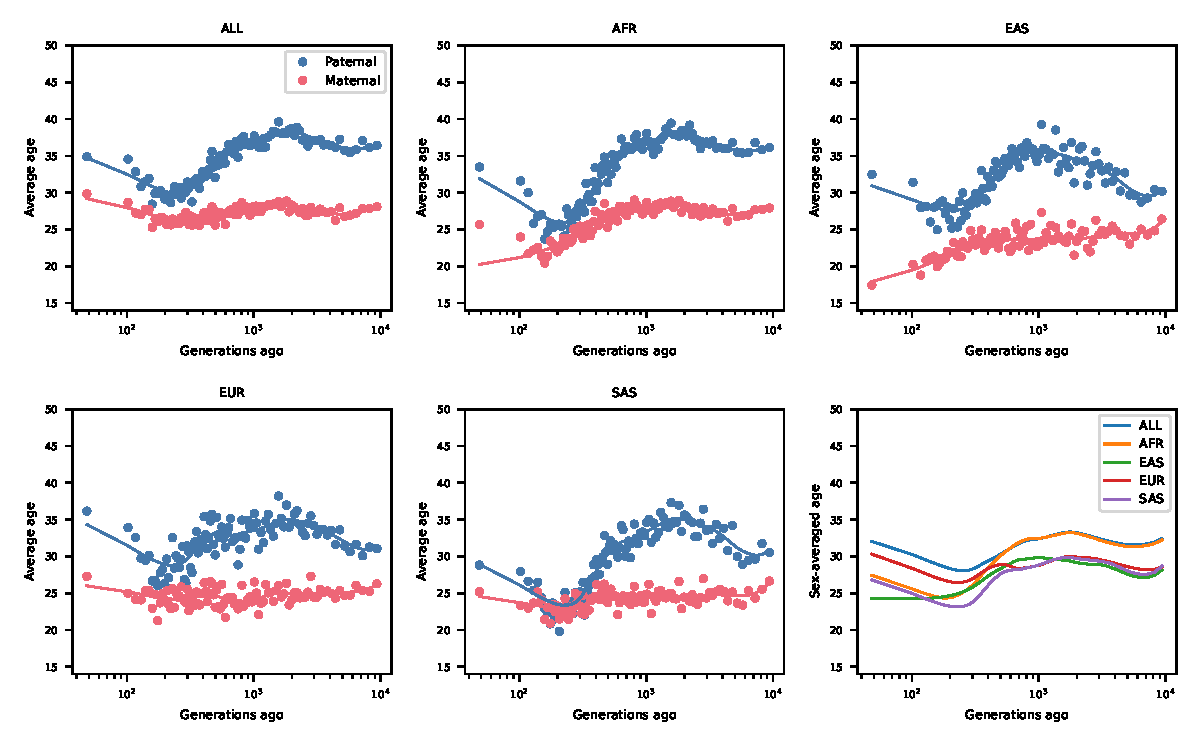
\includegraphics[width=\textwidth]{../plots/inferred_generation_times.DM.geva.max_age.10000.pdf}
    \caption{
        \textbf{\GEVA-inferred generation time histories.}
    }
    \label{fig:geva-gen-times}
\end{figure}

\begin{figure}[ht!]
    \centering
    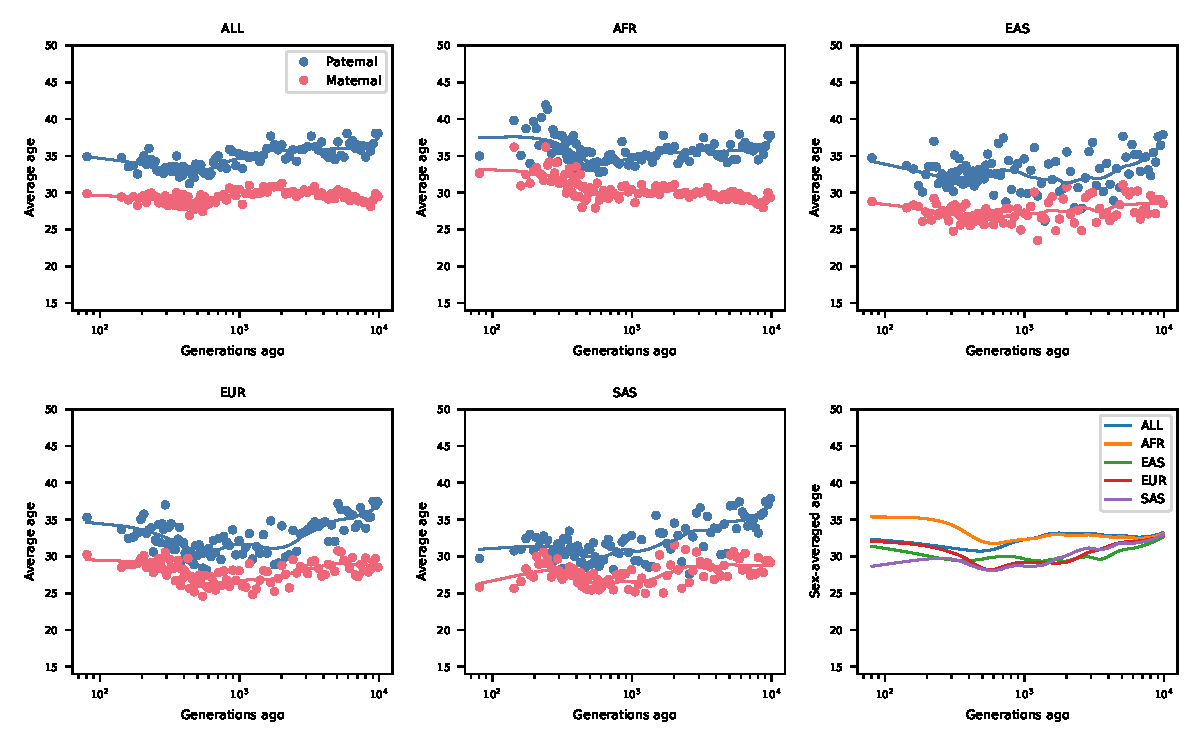
\includegraphics[width=\textwidth]{../plots/inferred_generation_times.DM.relate.max_age.10000.pdf}
    \caption{
        \textbf{\relate-inferred generation time histories.}
    }
    \label{fig:relate-gen-times}
\end{figure}


\begin{figure}[ht!]
    \centering
    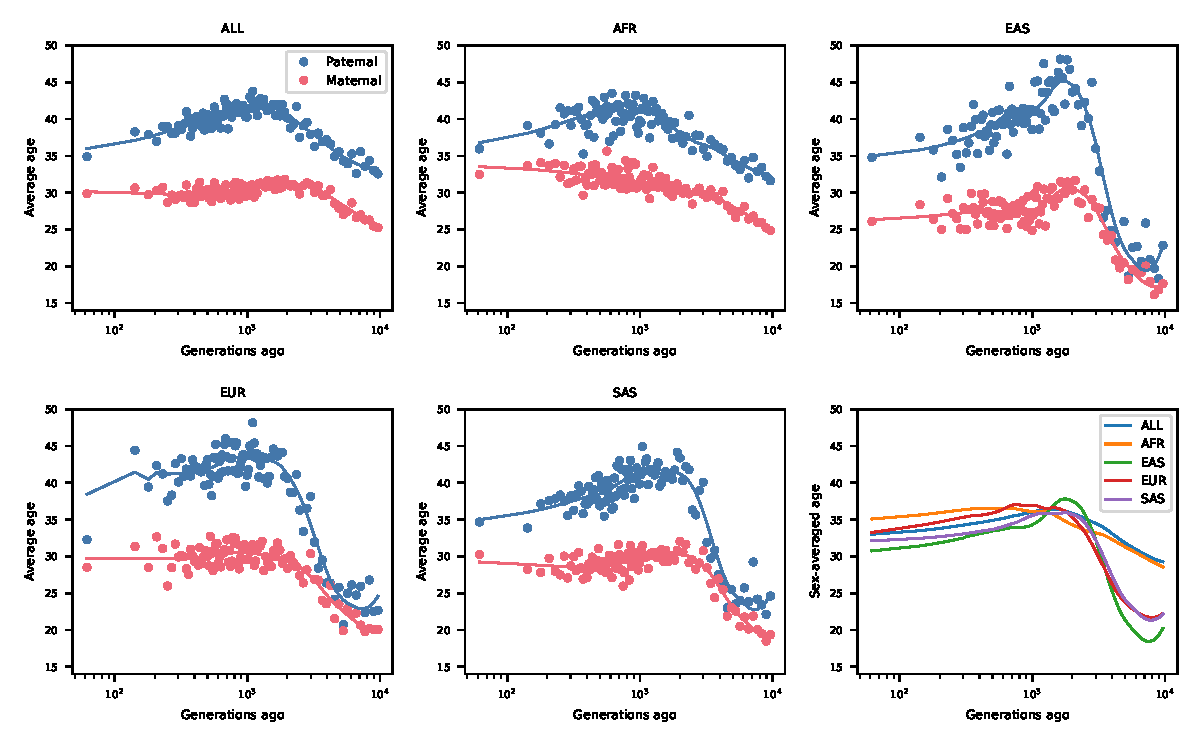
\includegraphics[width=\textwidth]{../plots/inferred_generation_times.DM.tsdate.max_age.10000.pdf}
    \caption{
        \textbf{\tsdate-inferred generation time histories.}
    }
    \label{fig:tsdate-gen-times}
\end{figure}


\begin{figure}[ht!]
    \centering
    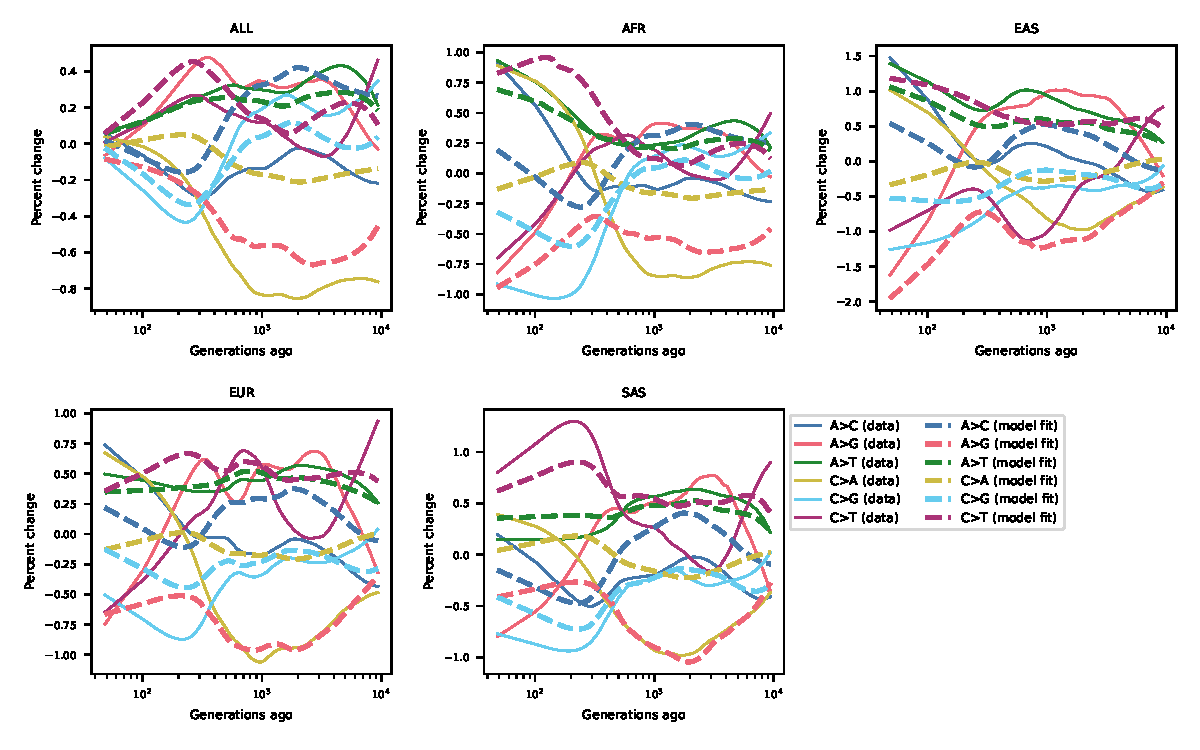
\includegraphics[width=\textwidth]{../plots/goodness-of-fit.DM.geva.max_age.10000.pdf}
    \caption{
        \textbf{Prediction of mutation spectrum history from
        \GEVA-inferred generation times.}
    }
    \label{fig:geva-fit}
\end{figure}

\begin{figure}[ht!]
    \centering
    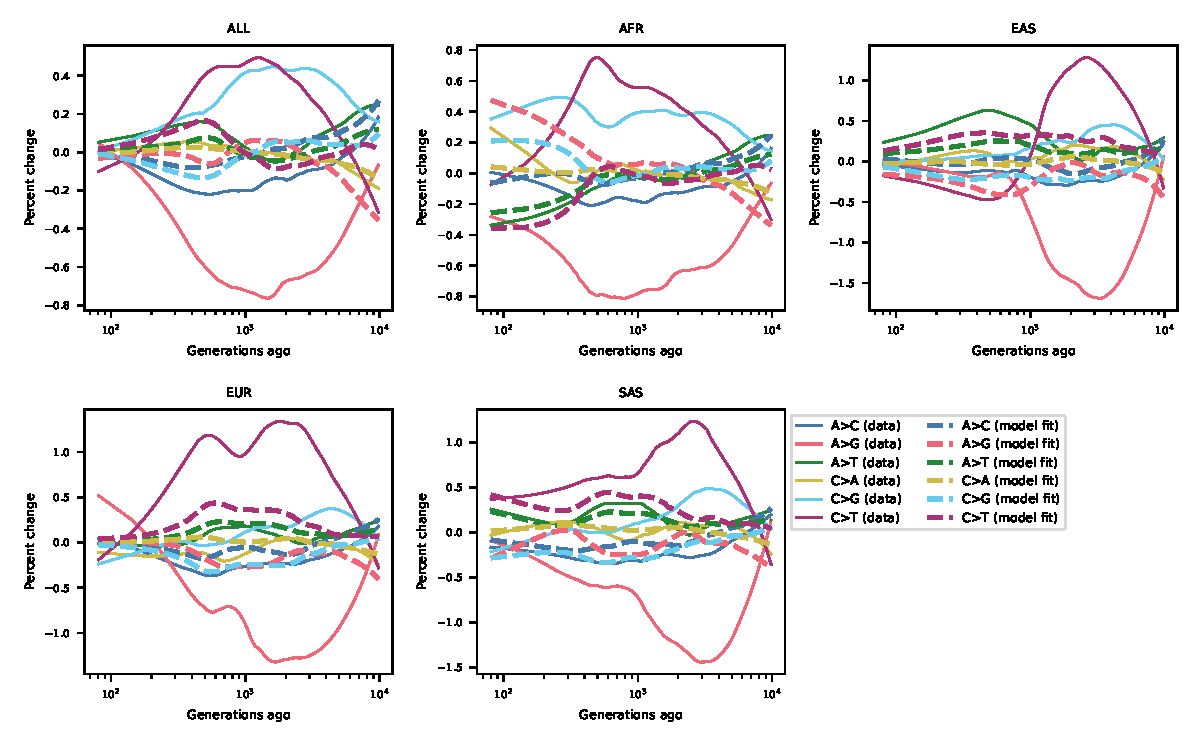
\includegraphics[width=\textwidth]{../plots/goodness-of-fit.DM.relate.max_age.10000.pdf}
    \caption{
        \textbf{Prediction of mutation spectrum history from
        \relate-inferred generation times.}
    }
    \label{fig:relate-fit}
\end{figure}


\begin{figure}[ht!]
    \centering
    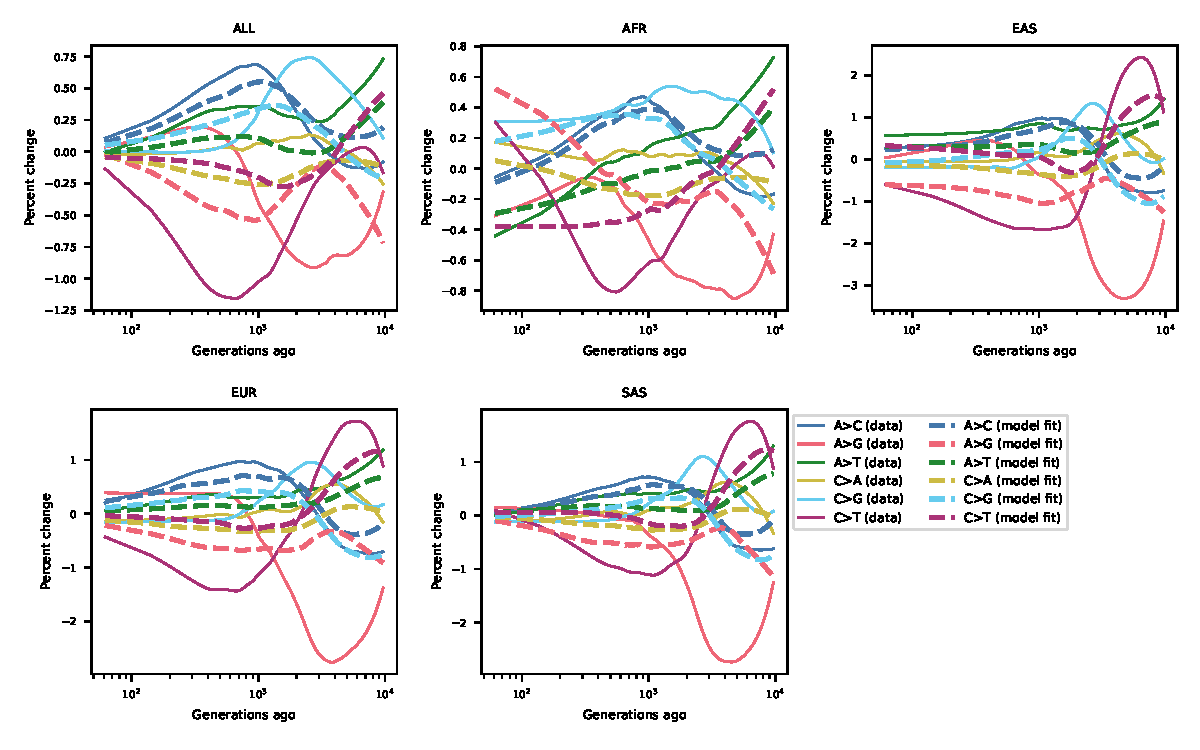
\includegraphics[width=\textwidth]{../plots/goodness-of-fit.DM.tsdate.max_age.10000.pdf}
    \caption{
        \textbf{Prediction of mutation spectrum history from
        \tsdate-inferred generation times.}
    }
    \label{fig:tsdate-fit}
\end{figure}


\break

\end{document}
